% DO NOT COMPILE THIS FILE DIRECTLY!
% This is included by the the driver file (FlipBeamerTemplate.tex).

{ %% This is a total kludge for a fancy title page background
%\setbeamertemplate{sidebar right}{\llap{\includegraphics[width=\paperwidth,height=\paperheight]{BG_upper}}}
\begin{frame}[c]%{\phantom{title page}} 
% The \phantom{title page} is a kludge to get the red bar on top
 \titlepage
\end{frame}
}

\begin{frame}
\frametitle{\textit{Background}}
Let 
\[
Y = \left(y_1,\dots, y_p\right)', \quad \left(t_1,\dots, t_p\right)'
\]
denote the random vector of observations and their associated measurement times, where 
\begin{align*}
 Cov\left(Y\right) = \Sigma = \left[ \sigma_{ij} \right] 
\end{align*}

\begin{itemize}
\item \nt{Dimensionality: the number of parameters is quadratic in $p$.} \pause
\item \nt{Covariance estimates should satisfy the positive definite constraint:}
\begin{equation*}
 		c'\Sigma c = \sum_{i,j = 1}^p c_i c_j \sigma_{ij} \ge 0
\end{equation*} \pause
\item \nt{Observation times may be irregular or subject-specific.} 
\end{itemize}
\end{frame}




\begin{frame}
\frametitle{\emph{The Modified Cholesky decomposition}}
For any positive definite $\Sigma$, there exists a unique lower-triangular matrix $C =  \left[c_{ij} \right]$, $c_{ii}> 0$:

\begin{equation*}
\Sigma = CC',
\end{equation*}

Let $D^{1/2} = diag\left( c_{11},\dots, c_{pp} \right)$, $L = D^{-1/2}C$, then 

\begin{equation*}
\Sigma =L D L'. %= CD^{-1/2}DD^{-1/2}C' = 
\end{equation*}

The \nt{\textbf{modified Cholesky decomposition} (MCD)} of $\Sigma$ is given by
\nt{\begin{equation}\label{eq:modified-cholesky-decomposition}
D = T\Sigma T',
\end{equation}}
where {$T = L^{-1}$}. The lower triangular entries of $T$ are \textit{unconstrained}.

\end{frame}





\begin{frame}
\frametitle{\emph{Statistical Interpretation of $\left(T,D\right)$}}{}
\footnotesize
Let $\hat{y}_t$ be the linear least-squares predictor of $y_t$ based on previous measurements $y_{t-1}, \dots , y_1$ and $\epsilon_t = y_t - \hat{y}_t$ denote the corresponding mean zero prediction error with variance $Var\left(\epsilon_t\right) = \sigma_t^2$. We can find unique scalars $\phi_{tj}$:

\nt{\begin{equation*} \label{eq:mcd-ar-model}
y_t = \left\{ \begin{array}{ll} \epsilon_t, & t = 1\\
\sum_{j = 1}^{t-1} \phi_{tj} y_j + \epsilon_t, & t = 2, \dots, p,
\end{array}\right.
\end{equation*}}

where $D = Cov\left( \epsilon \right) = diag\left( \sigma_1^2,\dots,\sigma_p^2, \right)$. Then

\begin{align*}
\underbrace{\begin{bmatrix}
\epsilon_1 \\
\epsilon_2 \\ \vdots \\\epsilon_{p-1} \\ \epsilon_p
\end{bmatrix}}_{\nt{\epsilon}} = \underbrace{\begin{bmatrix}
1&&&&\\
-\phi_{21}&1&&&\\
-\phi_{31}&-\phi_{32}&1&&\\
\vdots &&&\ddots& \\
-\phi_{p1}&-\phi_{p2}& \dots & -\phi_{p,p-1}&1\\
\end{bmatrix}}_{\nt{T}}
\underbrace{\begin{bmatrix}
y_1 \\
y_2 \\ \vdots \\ y_{p-1}\\y_p
\end{bmatrix}}_{\nt{Y}}
\end{align*}

Taking the covariance on both sides gives the \nt{MCD \eqref{eq:modified-cholesky-decomposition}}.
\end{frame}


\begin{frame}{\textit{The coefficients and prediction error variances of successive regressions are unconstrained.}}{}
\begin{columns}[T]
\begin{column}{0.5\textwidth}
The \textbf{generalized autoregressive parameters} $\phi_{tj}$ and \textbf{log innovation variances} $\log \sigma_j^2$ are unconstrained but  
\[
\hat{\Sigma}^{-1} = \hat{T}' \hat{D}^{-1} {T}
\]
is guaranteed to be positive definite.
\end{column}
\begin{column}{0.5\textwidth}
\footnotesize
\begin{tabular}{cccccc}
 $y_{1}$&$y_{2}$ & $y_{3}$ & $\dots$ &$y_{p-1}$& $y_{p}$\\ \hline
 $1$& &&&&\\
$\phi_{21}$& $1$ &&&& \\
$\phi_{31}$& $\phi_{32}$& $1$ &&& \\ 
$\vdots$ & $\vdots$ & & $\ddots$&& \\
$\vdots$ & $\vdots$ & && $\ddots$& \\
$\phi_{p1}$& $\phi_{p2}$&$\dots$ &$\dots$ &$\phi_{p,p-1}$ & $1$\\ \hline
$\sigma_1^2$ & $\sigma_2^2$ & $\dots$&$\dots$ &$\sigma_{p-1}^2$ &$\sigma_p^2$
\end{tabular} 
\end{column}
\end{columns}

\end{frame}











%\begin{frame}{Accommodating Unbalanced Data}{Subjects 1 and 2 have different measurement times.}
%
%  \begin{tikzpicture}
%    \node (yend) at (-0.35, 5.5)  {};
%    \node (xend) at ( 5.5, -0.35)  {};
%    \node at (0,6) {$1$};
%    \node at (1,5) {$1$};
%    \node at (2,4) {$1$};
%    \node at (3,3) {$1$};
%    \node at (4,2) {$1$};
%    \node at (5,1) {$\ddots$};
%    \node at (6,0) {$1$};
%     \node at (0,6) {$1$};
%    \node at (5,5.5) {\textcolor{paleale}{$t_1 = \left( t_{11}, t_{12}, \dots, t_{1p_1} \right)'$}};
%     \node at (5,5) {\textcolor{pink}{$t_2 = \left( t_{21}, t_{22}, \dots, t_{2p_2} \right)'$}};
%    \path[top color=gray, bottom color=gray!60] (-0.35,-0.35) -- (-0.35,5.85)  -- (5.85,-0.35) --  (-0.35,-0.35);
% \fill [white] (0,0.7) circle [radius=1pt];
% \fill [white] (0,1) circle [radius=1pt]; 
%  \fill [white] (0,1.3) circle [radius=1pt]; 
%  \node at (2,1) {\textcolor{mint}{$\left( t_{ij}, t_{ik}\right):\; t_{ij} > t_{ik}$}};
% \node at (4,2) {$1$};
%  \node at (4,2) {$1$};
%
%    \fill[white] (2.9,0) circle [radius=1pt];
%  \fill[white] (3.5,0) circle [radius=1pt]; 
%  \fill[white] (4.1,0) circle [radius=1pt]; 
%  
%  \fill[paleale]  (0,4.8) circle [radius=2.5pt];
%    \fill [paleale]  (0,4) circle [radius=2.5pt];
% \fill [paleale]  (0,2.5) circle [radius=2.5pt];
%   \fill[paleale]  (1.2,2.5) circle [radius=2.5pt];
%       \fill[paleale]  (2,2.5) circle [radius=2.5pt];
%  \fill[paleale] (0,2) circle [radius=2.5pt];
%   \fill[paleale] (1,2) circle [radius=2.5pt];
%       \fill[paleale] (2.5,2) circle [radius=2.5pt];
%    \fill[paleale] (0,0)  circle [radius=2.5pt];
%    \fill[paleale] (1.2,0)  circle [radius=2.5pt];
%       \fill[paleale] (2,0) circle [radius=2.5pt];
%    \fill[paleale] (5,0) circle [radius=2.5pt];
%    \fill[paleale] (1.2,4) circle [radius=2.5pt];
%      \fill[paleale]  (0,4.8) circle [radius=2.5pt];     
%
% \fill [pink]  (0.2,5) circle [radius=2.5pt];
%  \fill [pink]  (0.2,4) circle [radius=2.5pt];
% \fill [pink]  (0.2,3) circle [radius=2.5pt];
%   \fill[pink] (0.2,2.3) circle [radius=2.5pt];
%       \fill[pink] (0.2,0.3)  circle [radius=2.5pt];
%           \fill[pink] (1,0.3)  circle [radius=2.5pt];
%   \fill[pink]  (1,2.3) circle [radius=2.5pt];
%    \fill[pink] (1,3) circle [radius=2.5pt];
%    \fill[pink] (1,4) circle [radius=2.5pt];
%%   \fill[pink] (2, 1) circle [radius=2.5pt];
%  \fill[pink] (2,0.3) circle [radius=2.5pt];
%  \fill[pink] (2.7,2.3) circle [radius=2.5pt];
%    \fill[pink] (5,.3) circle [radius=2.5pt];
%\draw[<-, color = mint] (-0.55,-0.55) -- (-0.55,5.85); 
%\draw[->, color = mint] (-0.55,-0.65) -- (5.95,-0.65); 
%% \node at (0,5) {$\phi_{21}$};
%%   \node at (0,4) {$\phi_{31}$};
%% \node at (0,3) {$\phi_{41}$};
%%  \node at (1,3) {$\phi_{42}$};
%%   \node at (2,3) {$\phi_{43}$};
%% \node at (0,2) {$\phi_{51}$};
%%  \node at (1,2) {$\phi_{52}$};
%%      \node at (3,2) {$\phi_{54}$};
%%   \node at (0,0) {$\phi_{p1}$};
%%   \node at (1,0) {$\phi_{p2}$};
%%      \node at (2,0) {$\phi_{p3}$};
%%   \node at (5,0) {$\phi_{p, p-1}$};
%%      \node at (1,4) {$\phi_{32}$};
%%        \node at (2,2) {$\phi_{53}$};
%%    \node at (2,0) {$\phi_{p3}$};
%%   \node at (5,0) {$\phi_{p, p-1}$};
% \node at (-0.75,2.5) {\textcolor{mint}{$t$}};
%  \node at (2.5,-0.85) {\textcolor{mint}{$s$}};
%   \end{tikzpicture} \\
%\end{frame}
%
%
%
%
%
%\begin{frame}{Accommodating Unbalanced Data}{Subjects 1 and 2 have different measurement times.}
%
%  \begin{tikzpicture}
%    \node (yend) at (-0.35, 5.5)  {};
%    \node (xend) at ( 5.5, -0.35)  {};
%    \node at (0,6) {$1$};
%    \node at (1,5) {$1$};
%    \node at (2,4) {$1$};
%    \node at (3,3) {$1$};
%    \node at (4,2) {$1$};
%    \node at (5,1) {$\ddots$};
%    \node at (6,0) {$1$};
%    \path[top color=gray, bottom color=gray!60] (-0.35,-0.35) -- (-0.35,5.85)  -- (5.85,-0.35) --  (-0.35,-0.35);
% \fill [white] (0,0.7) circle [radius=1pt];
% \fill [white] (0,1) circle [radius=1pt]; 
%  \fill [white] (0,1.3) circle [radius=1pt]; 
%
%    \fill[white] (2.9,0) circle [radius=1pt];
%  \fill[white] (3.5,0) circle [radius=1pt]; 
%  \fill[white] (4.1,0) circle [radius=1pt]; 
%  
%  \fill[paleale]  (0,4.8) circle [radius=2.5pt];
%    \fill [paleale]  (0,4) circle [radius=2.5pt];
% \fill [paleale]  (0,2.5) circle [radius=2.5pt];
%   \fill[paleale]  (1.2,2.5) circle [radius=2.5pt];
%       \fill[paleale]  (2,2.5) circle [radius=2.5pt];
%  \fill[paleale] (0,2) circle [radius=2.5pt];
%   \fill[paleale] (1,2) circle [radius=2.5pt];
%       \fill[paleale] (2.5,2) circle [radius=2.5pt];
%    \fill[paleale] (0,0)  circle [radius=2.5pt];
%    \fill[paleale] (1.2,0)  circle [radius=2.5pt];
%       \fill[paleale] (2,0) circle [radius=2.5pt];
%    \fill[paleale] (5,0) circle [radius=2.5pt];
%    \fill[paleale] (1.2,4) circle [radius=2.5pt];
%      \fill[paleale]  (0,4.8) circle [radius=2.5pt];     
%
% \fill [pink]  (0.2,5) circle [radius=2.5pt];
%  \fill [pink]  (0.2,4) circle [radius=2.5pt];
% \fill [pink]  (0.2,3) circle [radius=2.5pt];
%   \fill[pink] (0.2,2.3) circle [radius=2.5pt];
%       \fill[pink] (0.2,0.3)  circle [radius=2.5pt];
%           \fill[pink] (1,0.3)  circle [radius=2.5pt];
%   \fill[pink]  (1,2.3) circle [radius=2.5pt];
%    \fill[pink] (1,3) circle [radius=2.5pt];
%    \fill[pink] (1,4) circle [radius=2.5pt];
%%   \fill[pink] (2, 1) circle [radius=2.5pt];
%  \fill[pink] (2,0.3) circle [radius=2.5pt];
%  \fill[pink] (2.7,2.3) circle [radius=2.5pt];
%    \fill[pink] (5,.3) circle [radius=2.5pt];
%
% \node at (0,5) {$\phi_{21}$};
%   \node at (0,4) {$\phi_{31}$};
% \node at (0,3) {$\phi_{41}$};
%  \node at (1,3) {$\phi_{42}$};
%   \node at (2,3) {$\phi_{43}$};
% \node at (0,2) {$\phi_{51}$};
%  \node at (1,2) {$\phi_{52}$};
%      \node at (3,2) {$\phi_{54}$};
%   \node at (0,0) {$\phi_{p1}$};
%   \node at (1,0) {$\phi_{p2}$};
%      \node at (2,0) {$\phi_{p3}$};
%   \node at (5,0) {$\phi_{p, p-1}$};
%      \node at (1,4) {$\phi_{32}$};
%        \node at (2,2) {$\phi_{53}$};
%    \node at (2,0) {$\phi_{p3}$};
%   \node at (5,0) {$\phi_{p, p-1}$};
%    \node at (-0.75,2.5) {\textcolor{mint}{$t$}};
%  \node at (2.5,-0.85) {\textcolor{mint}{$s$}};
%   \draw[<-, color = mint] (-0.55,-0.55) -- (-0.55,5.85); 
%\draw[->, color = mint] (-0.55,-0.65) -- (5.95,-0.65); 
%   \end{tikzpicture} \\
%\end{frame}
%


\begin{frame}{Accommodating Unbalanced Data}{Treating $\phi$ as a continuous bivariate function.}

  \begin{tikzpicture}
    \node (yend) at (-0.35, 5.5)  {};
    \node (xend) at ( 5.5, -0.35)  {};
    \node at (0,6) {$1$};
    \node at (1,5) {$1$};
    \node at (2,4) {$1$};
    \node at (3,3) {$1$};
    \node at (4,2) {$1$};
    \node at (5,1) {$\ddots$};
    \node at (6,0) {$1$};
    \path[top color=gray, bottom color=gray!60] (-0.35,-0.35) -- (-0.35,5.85)  -- (5.85,-0.35) --  (-0.35,-0.35);
    \node at (0,5) {$\phi_{21}$};
   \node at (0,4) {$\phi_{31}$};
 \node at (0,3) {$\phi_{41}$};
 \fill [white] (0,0.7) circle [radius=1pt];
 \fill [white] (0,1) circle [radius=1pt]; 
  \fill [white] (0,1.3) circle [radius=1pt]; 
  \node at (1,3) {$\phi_{42}$};
   \node at (2,3) {$\phi_{43}$};
 \node at (0,2) {$\phi_{51}$};
  \node at (1,2) {$\phi_{52}$};
      \node at (3,2) {$\phi_{54}$};
   \node at (0,0) {$\phi_{p1}$};
   \node at (1,0) {$\phi_{p2}$};
      \node at (2,0) {$\phi_{p3}$};
   \node at (5,0) {$\phi_{p, p-1}$};
    \fill [white] (2.9,0) circle [radius=1pt];
 \fill [white] (3.5,0) circle [radius=1pt]; 
  \fill [white] (4.1,0) circle [radius=1pt]; 
   \node at (1,4) {$\phi_{32}$};
\draw[<-, color = mint] (-0.55,-0.55) -- (-0.55,5.85); 
\draw[->, color = mint] (-0.55,-0.65) -- (5.95,-0.65); 
 \node at (-0.75,2.5) {\textcolor{mint}{$t$}};
  \node at (2.5,-0.85) {\textcolor{mint}{$s$}};
       \node at (2,0) {$\phi_{p3}$};
   \node at (5,0) {$\phi_{p, p-1}$};
%   \fill [mint] (2,2) circle [radius=2pt];
%    \path[->, color=mint, line width=1] (2,2) edge [out = 50,in = 160] (6,5);
% \node at (7.5,5) {\textcolor{mint}{$\phi_{54} = \phi\left(t_5,t_4\right)$}};
   \end{tikzpicture} \\
\end{frame}


\begin{frame}{Accommodating Unbalanced Data}{Treating $\phi$ as a continuous bivariate function.}

  \begin{tikzpicture}
    \node (yend) at (-0.35, 5.5)  {};
    \node (xend) at ( 5.5, -0.35)  {};
    \node at (0,6) {$1$};
    \node at (1,5) {$1$};
    \node at (2,4) {$1$};
    \node at (3,3) {$1$};
    \node at (4,2) {$1$};
    \node at (5,1) {$\ddots$};
    \node at (6,0) {$1$};
    \path[top color=gray, bottom color=gray!60] (-0.35,-0.35) -- (-0.35,5.85)  -- (5.85,-0.35) --  (-0.35,-0.35);
    \node at (0,5) {$\phi_{21}$};
   \node at (0,4) {$\phi_{31}$};
 \node at (0,3) {$\phi_{41}$};
 \fill [white] (0,0.7) circle [radius=1pt];
 \fill [white] (0,1) circle [radius=1pt]; 
  \fill [white] (0,1.3) circle [radius=1pt]; 
  \node at (1,3) {$\phi_{42}$};
   \node at (2,3) {$\phi_{43}$};
 \node at (0,2) {$\phi_{51}$};
  \node at (1,2) {$\phi_{52}$};
      \node at (3,2) {$\phi_{54}$};
   \node at (0,0) {$\phi_{p1}$};
   \node at (1,0) {$\phi_{p2}$};
      \node at (2,0) {$\phi_{p3}$};
   \node at (5,0) {$\phi_{p, p-1}$};
    \fill [white] (2.9,0) circle [radius=1pt];
 \fill [white] (3.5,0) circle [radius=1pt]; 
  \fill [white] (4.1,0) circle [radius=1pt]; 
   \node at (1,4) {$\phi_{32}$};
\draw[<-, color = mint] (-0.55,-0.55) -- (-0.55,5.85); 
\draw[->, color = mint] (-0.55,-0.65) -- (5.95,-0.65); 
 \node at (-0.75,2.5) {\textcolor{mint}{$t$}};
  \node at (2.5,-0.85) {\textcolor{mint}{$s$}};
       \node at (2,0) {$\phi_{p3}$};
   \node at (5,0) {$\phi_{p, p-1}$};
   \fill [mint] (2,2) circle [radius=2pt];
    \path[->, color=mint, line width=1] (2,2) edge [out = 50,in = 160] (6,5);
 \node at (7.5,5) {\textcolor{mint}{$\phi_{53} = \tilde{\phi}\left(t_5,t_3\right)$}};
  \node at (7.3,3.4) {\footnotesize\textcolor{mint}{In general, $\phi_{ts}= \tilde{\phi}\left(t,s\right), \;\;\;\;0 \le s < t \le 1$}};
  \node at (7.7,2.7) {\footnotesize\textcolor{mint}{ $\sigma^2_{t} = \sigma^2\left(t\right), \;\;\;\;0 \le t \le 1$}};
%  \node at (7.8,3.5) {\footnotesize\textcolor{mint}{$\phi_{ts} = \tilde{\phi}\left(t,s\right), \quad 0 \le s < t \le 1$}};
%    \node at (7.4,3) {\footnotesize\textcolor{mint}{$\sigma^2_{t} = \sigma^2\left(t\right), \quad 0 \le s t \le 1$}};
   \end{tikzpicture} \\
\end{frame}



\begin{frame}{\textit{A functional varying coefficient model for} $\phi$ }%{A Bivariate Functional Varying-Coefficient Model for $\phi$}
\footnotesize
Assume measurements $Y_i = \left(y_{i1}, \dots, y_{i,p_i}\right)'$ arise from $Y\left(t\right)$ observed at 
\[
t_{i} = \left\{t_{i1} <  \dots < t_{i,p_i}\right\} \subset \mathcal{T} = \left[0,1\right]
\]
%\nt{\begin{equation*}
%{y\left(t_{ij} \right)  = \sum_{k < j} \tilde{\phi}\left(t_{ij} ,t_{ik}\right) y\left(t_{ik}\right) + \epsilon\left({t_{ij}}\right), \quad \begin{array}{l} i = 1, \dots, N\\ j = 2, \dots, p_i,\end{array}}
%\end{equation*}
%}
\nt{\begin{empheq}[box=\fbox]{align}
{y\left(t_{ij} \right)  = \sum_{k < j} \tilde{\phi}\left(t_{ij} ,t_{ik}\right) y\left(t_{ik}\right) + \epsilon\left({t_{ij}}\right), \quad \begin{array}{l} i = 1, \dots, N\\ j = 2, \dots, p_i,\end{array}} \nonumber
\end{empheq}}
where $\epsilon\left(t\right) \sim N\left(0,\sigma^2\left(t\right)\right)$. Transform $l = t - s, \quad m = \frac{t + s}{2}$, let
\nt{\begin{align*}%\label{eq:l-m-transformation}
 \phi\left(l,m\right) = {\phi}\left(t-s, \frac{1}{2}\left(s+t\right)\right) = \tilde{\phi}\left(t,s\right),
\end{align*}}
so that \footnotesize
\begin{equation*} \label{eq:full-joint-likelihood}
-2\ell\left(\phi, \sigma^2 \vert Y_1,\dots, Y_N \right) = \sum_{i=1}^N \sum_{j=2}^{p_i} \left[ \log \sigma_{ij}^2+ \frac{1}{\sigma^{2}_{ij}}\left( y_{ij} - \sum_{k<j} \tilde{\phi}\left(t_{ij}, t_{ik}\right) y_{ik}  \right)^2\right]
\end{equation*}
\end{frame}


%%%%%%%%%%%%%%%%%%%%%%%%%%%%%%%%%%%%%%%%%%%%%%%%%%%%%%%%%%%%%%%%%%%%%%%%%%%%
%%%%%%%%%%%%%%%%%%%%%%%%%%%%%%%%%%%%%%%%%%%%%%%%%%%%%%%%%%%%%%%%%%%%%%%%%%%%
%%%%%%%%%%%%%%%%%%%%%%%%%%%%%%%%%%%%%%%%%%%%%%%%%%%%%%%%%%%%%%%%%%%%%%%%%%%%
%%%%%%%%%%%%%%%%%%%%%%%%%%%%%%%%%%%%%%%%%%%%%%%%%%%%%%%%%%%%%%%%%%%%%%%%%%%%

\begin{frame}{\textit{Hilbert spaces for univariate functions}}{An example: the cubic smoothing spline}
\begin{small}
The cubic smoothing spline corresponds to model space
\begin{equation*}
\hilbert = W_2[0,1]=\{f:[0,1]\rightarrow \Bbb{R}~| f, ~f' \mbox{ abs cnts, } \int (f''(x))^2 dx<\infty\}.
\end{equation*}
and is the solution to the penalized least squares problem with
\begin{equation*}
J(f)=\int_0^1 (f''(x))^2 dx.
\end{equation*}
Equip $\hilbert$ with inner product such that 
\nt{$\hilbert = {\hilbert_0} \oplus \hilbert_1$ where $J\left(f\right) = 0$ for $f \in \hilbert_0$.}
\begin{itemize}
\item $\hilbert$ has corresponding reproducing kernel $K = K_0 + K_1$.
\item Take functions in \nt{null space} $\hilbert_0 = \lbrace \mbox{linear or constant functions} \rbrace$ to be null models.
\item \nt{$J(f) = \| P_1f\|^2$} corresponds to the squared norm of the projection of $f$ to $\hilbert_1$. 
\end{itemize}
\end{small}
\end{frame}

\begin{frame}{\textit{One-way functional ANOVA models}}{}
\begin{small}
Given
\begin{enumerate}
\item averaging operator $A(f)=\int_0^1 f(x) dx$,
\item basis $k_1(\cdot)$ for linear functions in $\hilbert_0$ such that $A(k_1) = 0$, 
\end{enumerate}
$\hilbert$ admits decomposition
\begin{align*}
\hilbert &=  {\{1\}}  \oplus  \{k_1(\cdot)\} \oplus {\hilbert_1} \\
&= \text{\footnotesize{mean}} \oplus {\substack{\text{parametric} \\ \text{main effect}}} \oplus {\substack{\text{nonparametric} \\ \text{main effect}}}
\end{align*}
and representation
\begin{equation*}
f\left(x\right) = c_0+c_1k_1(x)+f_1(x); \quad f \in \hilbert
\end{equation*}
where $c_0, c_1 \in \Bbb{R}$ and $f_1\in \hilbert_1$.
\end{small}
\end{frame}


\begin{frame}{\textit{A Two-way functional ANOVA Model for $\phi$}}{via tensor product}
\begin{small} Let
\[
\phi \in \hilbert = \hilbert^{[l]} \otimes \hilbert^{[m]}
\]
constructed from building blocks
\begin{align*}
\hilbert^{[l]} &=\{1\}\oplus \{k_1(l)\} \oplus \hilbert_1^{[l]} \\
\hilbert^{[m]} &=\{1\}\oplus \hilbert_1^{[m]}. 
\end{align*} 
with RK $K$. The subspaces of $\hilbert$ define unique decomposition
\[
\nt{\phi(l,m)=\mu+\phi_1(l)+\phi_2(m)+\phi_{12}(l,m).}
\]
\begin{tabular}{r|c|c|c|} % centered columns (4 columns)
\multicolumn{1}{c}{} & \multicolumn{1}{c}{	$\left\{1\right\}$}	&	\multicolumn{1}{c}{$ \left\{k_1\right\}$}	&\multicolumn{1}{c}{ $\hilbert^{\left[l\right]}_{1}$}\\ [1.5ex] 
\cline{2-4}  % inserts single horizontal line\\
$ \left\{1\right\}$		& mean	&	$p$-main effect	&	$np$-main effect  \\  
 $\hilbert^{\left[m\right]}_{1}$	& 	$np$-main effect 	&  $np\times p$-interaction	&	$np \times np$-interaction \\
\cline{2-4}
\end{tabular}
\end{small}
\end{frame}


\begin{frame}{\textit{Penalized log likelihood for $\phi$}}{}
\small
Define transformed pairs of observation times
\begin{align*}
\bfv_{ijk} &= (t_{ij} - t_{ik}, \frac{1}{2}\left(t_{ij} + t_{ik}\right)) = \left(l_{ijk}, m_{ijk}\right),\\
V &= \bigcup\limits_{i,j,k} \left\{\bfv_{ijk} \right\} = \left\{ \bfv_1,\dots,\bfv_{\vert V \vert} \right\}.
\end{align*}
Fixing $\sigma_{ij}^2 = \sigma^2\left(t_{ij}\right)$, find $\phi$ minimizing
\nt{ \footnotesize
\begin{equation} \label{eq:phi-penalized-sums-of-squares}
-2\ell\left(\phi \vert Y_1,\dots, Y_N, \sigma^2\right) + \lambda J\left(\phi\right) = \sum_{i=1}^N \sum_{j=2}^{p_i} \frac{1}{\sigma^{2}_{ij}}\left( y_{ij} - \sum_{k<j}\phi\left(\bfv_{_{ijk}}\right) y_{ik}  \right)^2 + \lambda J\left(\phi\right) 
\end{equation}} 
\small
where $J\left(\phi\right) =\vert \vert P_1 \phi \vert\vert^2$ and $\bfv_{ijk} \in \mathcal{V} = \left[0,1\right]^2$, 

\end{frame}

\begin{frame}{\textit{A Representer Theorem}}{}

 \begin{theorem} \label{theorem:finite-dimensional-minimizer}
 Let $\left\{\nu_1,\dots, \nu_{\mathcal{N}_0}\right\}$ span $\hilbert_0$, the null space of $J\left(\phi\right) = \vert \vert P_1 \phi\vert\vert^2$. Let $B$ denote the $\vert V \vert \times \mathcal{N}_0$ matrix having $i^{th}$ column equal to $\nu_i$ evaluated at the observed $\bfv \in V$, and assume that $B$ has full column rank. Then the minimizer $\phi_\lambda$ of \eqref{eq:phi-penalized-sums-of-squares} is given by
 \begin{equation} \label{eq:form-of-the-minimizer-phi}
\phi_\lambda\left(\bfv\right) = \sum_{i = 1}^{\mathcal{N}_0} d_i \nu_{i}\left(\bfv\right) + \sum_{j = 1}^{\vert V \vert} c_j K_1\left(\bfv_j, \bfv\right),
\end{equation}
\noindent
where $K_1\left(\bfv_j, \bfv \right)$ denotes the reproducing kernel for $\hilbert_1$ evaluated at ${\bfv_j}$, the $j^{th}$ element of $V$.
\end{theorem}

\end{frame}


\begin{frame}{\textit{Obtaining the solution}  $\phi_\lambda$}
\footnotesize
By the Representer Theorem, \nt{\eqref{eq:phi-penalized-sums-of-squares}} becomes
\nt{ \begin{equation*}\label{eq:penalized-loglik-tilde-vectorized}
-2\ell \left(c, d \vert \tildeY, \tildeB, \tildeK_{_{ V}} \right) + \lambda J\left( \phi \right) = \bigg[ \tildeY - \tildeB d - \tildeK_{_{ V}} c\bigg]'\bigg[ \tildeY - \tildeB d - \tildeK_{_{ V}} c\bigg] + \lambda c'K_Vc,
\end{equation*}}\footnotesize
where
\begin{scriptsize}
\begin{align*}%\label{eq:stacked-response-vector}
Y&= \left( Y'_1, Y'_2, \dots, Y'_{N} \right)' = \left( y_{12}, y_{13},\dots, y_{1p_1}, \dots, y_{N2},\dots, y_{Np_N} \right)', \\
D &= diag\left( \sigma^2_{12}, \sigma^2_{13},\dots, \sigma^2_{1p_1}, \dots,\sigma^2_{N2},\dots, \sigma^2_{Np_N}  \right)\\
X &= \begin{bmatrix} X'_1 &X'_2 &  \dots & X'_N \end{bmatrix}' \\
X_i &= \left(p_i-1\right) \times \vert V \vert \mbox{ matrix of AR covariates for Subject }i ,\\
K_{_{ V}} &= \vert V \vert \times \vert V \vert \mbox{ matrix with } \left(i,j\right) \mbox{ element } K_1\left(\bfv_i, \bfv_j\right)\\
B &= \vert V \vert \times \mathcal{N}_0 \mbox{ matrix with } \left(i,j\right) \mbox{ element } \nu_j\left(\bfv_i\right)
\end{align*} 
\end{scriptsize}
\footnotesize
and $\tildeY = D^{-1/2} Y$, $\tildeB = D^{-1/2} X B $, $\tildeK_{_{ V}} = D^{-1/2} X K_{_{ V}}$.
\end{frame}


\begin{frame}{\textit{Obtaining the solution}  $\phi_\lambda$}
\footnotesize
Setting derivatives equal to zero, for fixed $\lambda$, $c$ and $d$ satisfy
\begin{align*}% \label{eq:vectorized-normal-equations}
\begin{bmatrix}
\tildeB'\tildeY \\
 \tildeK_{_{ V}}'\tildeY\\
\end{bmatrix} &= \underbrace{\begin{bmatrix}
\tildeB'\tildeB & \tildeB'\tildeK_{_{ V}} \\
\tildeK_{_{ V}}'\tildeB & \tildeK_{_{ V}}'\tildeK_{_{ V}} + \lambda K_{_{ V}}\\
\end{bmatrix}}_{C'C}
\begin{bmatrix}
d\\
c\\
\end{bmatrix}
\\
\Longrightarrow \begin{bmatrix} \hat{d} \\ \hat{c} \end{bmatrix} &=  {C}^{-1} ({C}')^{-1} \begin{bmatrix} \tildeB' \\ \tildeK_{_{ V}}' \end{bmatrix} \tildeY. 
\end{align*}

The fitted values are given by $\widehat{\tildeY} =  \tildeA_{\lambda,\bftheta} \tildeY$, where the smoothing matrix is
\nt{\begin{align*}
\tildeA_{\lambda,\bftheta} = \begin{bmatrix} \tildeB & \tildeK_{_{ V}} \end{bmatrix} {C}^{-1} ({C}')^{-1} \begin{bmatrix} \tildeB' \\ \tildeK_{_{ V}}' \end{bmatrix}  
\end{align*} }
and can be used to compute model selection criteria.
%\begin{align*}
%U\left(\lambda\right) &= \tildeY'\left( I - \tildeA_{\lambda,\bftheta} \right)^2\tildeY + {2}\mbox{ tr}\left(\tildeA_{\lambda,\bftheta}\right) \mbox{ or}\\
%V_{loso}\left(\lambda\right) &= \frac{1}{N}\sum_{i=1}^N \left( \tildeY_i - \widehat{\tilde{\mu}}^{\left[-i\right]}_{i}\right)'\left( \tildeY_i -  \widehat{\tilde{\mu}}^{\left[-i\right]}_{i}\right)
%\end{align*}
\end{frame}


\begin{frame}{\textit{A RKHS Framework for $\log \sigma^2$}}
For fixed $\phi\left(\cdot\right)$, let $Z_i = \left(z_{i1}, \dots , z_{ip_i}\right)'$, $z_{ij} = \epsilon_{ij}^2$, where
\[
\epsilon_{ij} =  y_{ij} - \sum_{k<j} \phi\left(\bfv_{ijk}\right) y_{ik}.
\]
The log likelihood of the squared working innovations $Z_1,\dots, Z_N$ coincides with a Gamma distribution with scale parameter $\alpha = 2$:
\begin{equation*} %\label{eq:penalized-joint-loglik-given-phi-3}
-2\ell\left(  \sigma^2 \vert Z_1,\dots, Z_N \right) =  \sum_{i = 1}^N \sum_{j = 1}^{p_i} \eta_{ij}  + \sum_{i = 1}^N \sum_{j = 1}^{p_i} z_{ij}e^{-\eta_{ij}},
\end{equation*}
\noindent
where $\eta_{ij} = \eta\left(t_{ij}\right) = \log \sigma^2\left(t_{ij}\right)$.
\end{frame}


\begin{frame}{\textit{A RKHS Framework for $\log \sigma^2$}}
\footnotesize
Take the estimator of $\eta\left(t\right) = \log\sigma^2\left(t\right) \in \hilbert$ to minimize
\begin{equation*} %\label{eq:penalized-joint-loglik-given-phi}
-2\ell\left( \eta \vert Z_1,\dots, Z_N \right) +\lambda J \left(\eta\right) =  \sum_{i = 1}^N \sum_{j = 1}^{p_i} \eta\left(t_{ij}\right)  + \sum_{i = 1}^N \sum_{j = 1}^{p_i} z_{ij} e^{-\eta\left(t_{ij}\right)} + \lambda J\left(\eta\right).  
\end{equation*}
\noindent
Let $\mathcal{T} = \bigcup_{i,j} \left\{t_{ij}\right\}$. By Theorem~\ref{theorem:finite-dimensional-minimizer}, the minimizer has the form 
\begin{equation*}% \label{eq:form-of-smoothing-spline-solution-kappa}
\eta_\lambda\left( t \right) = \sum_{i = 1}^{\mathcal{N}_0} d_i \nu_i\left( t \right) + \sum_{j = 1}^{\vert \mathcal{T} \vert} c_j K_1\left(t_j,t\right),
\end{equation*}  
\noindent
where $\left\{\nu_i \right\}$ span $\hilbert_0$, $K_1\left(t_j,t\right)$ is the RK for $\hilbert_1$ evalutated at ${t_j}$, the $j^{th}$ element of $\mathcal{T}$.

\end{frame}



%%%%%%%%%%%%%%%%%%%%%%%%%%%%%%%%%%%%%%%%%%%%%%%%%%%%%%%%%%%%%%%%%%%%%%%%%%%%
%%%%%%%%%%%%%%%%%%%%%%%%%%%%%%%%%%%%%%%%%%%%%%%%%%%%%%%%%%%%%%%%%%%%%%%%%%%%
%%%%%%%%%%%%%%%%%%%%%%%%%%%%%%%%%%%%%%%%%%%%%%%%%%%%%%%%%%%%%%%%%%%%%%%%%%%%
%%%%%%%%%%%%%%%%%%%%%%%%%%%%%%%%%%%%%%%%%%%%%%%%%%%%%%%%%%%%%%%%%%%%%%%%%%%%

\begin{frame}{\emph{Simulation Studies}}\label{simulation-studies-benchmark-estimators}
\footnotesize
\begin{enumerate}
\item Simulations with complete data varying 
	\begin{itemize}
	\item generating model $\Sigma$
	\item number of subjects $N = 50, 100$
	\item dimension $p = 10, 20, 30$
	\end{itemize}
to compare performance to the oracle estimator, \hyperlink{polynomial-mcd-model}{Polynomial MCD GLM} $\hat{\Sigma}_{poly}$, the sample covariance matrix $S = \left[s_{ij}\right]$, \hyperlink{shrinkage-estimators}{Shrinkage estimators} $S^\omega$, $S^\lambda$
\item Simulations with unbalanced data to study robustness to missing or irregular data
		\begin{itemize}
	\item generating model $\Sigma$
	\item dimension $p = 10, 20$
	\item proportion of missing data 10\%, 20\%, 30\%
	\end{itemize}
\end{enumerate}

\footnotesize
Use Monte Carlo simulation to estimate risk $R \left(\Sigma,\hat{\Sigma}\right) = E_\Sigma\left[\Delta\left(\Sigma,\hat{\Sigma}\right)\right]$ under loss functions	
	\[
	\Delta_1\left(\Sigma,\hat{\Sigma} \right) = tr\left(\left( \Sigma^{-1} \hat{\Sigma} - \mathrm{I}\right)^2 \right),\;\;	\Delta_2\left(\Sigma,\hat{\Sigma}\right) = tr\left( \Sigma^{-1} \hat{\Sigma} \right) - log \vert \Sigma^{-1} \hat{\Sigma} \vert - p
	%\end{equation}
	\]

\end{frame}


\begin{frame}[c]{\emph{Simulation Studies}}{Data Generation Models}

\begin{center}
  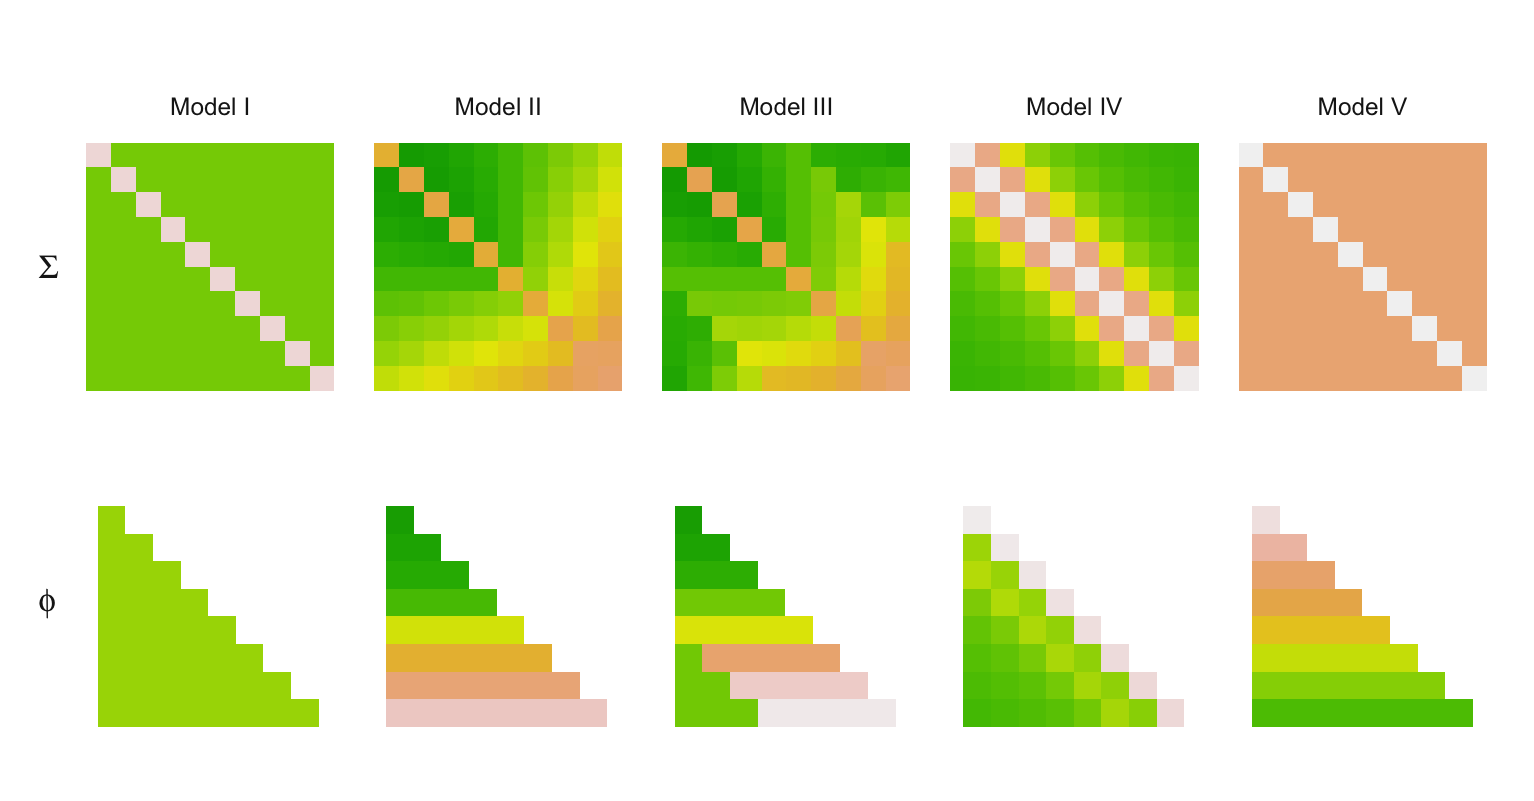
\includegraphics[width = \textwidth]{img/chapter-4/cov-cholesky-grid-beamer}%}
\end{center}
\end{frame}

\begin{frame}{\emph{Simulation Studies}}{Data Generation Settings}

\scriptsize
\begin{center}
\begin{tabular}{lll}
\textbf{I.}  $\Sigma = \mathrm{I}$ & $\phi\left(t,s\right) = 0$, $0 \le s < t \le1$ & $\sigma^2\left(t\right) = 1$, $0 \le  t \le1$\\
\\
\hline
\\
\textbf{II.}  $\Sigma = T^{-1} D {T'}^{-1}$ & $\phi\left(t,s\right) = t - \frac{1}{2},  \;\; 0 \le t \le 1$ & $\sigma^2\left(t\right) = 0.1^2$, $0 \le  t \le1$\\
\\
\hline
\\
\textbf{III.} $\Sigma = T^{-1} D {T'}^{-1}$ & $\phi\left(t,s\right) = \left\{\begin{array}{l} t - \frac{1}{2}, \;\; t - s \le 0.5\\  0, \;\;\;\;\;\; t - s > 0.5\end{array}\right.$ & $\sigma^2\left(t\right) = 0.1^2$, $0 \le  t \le1$ \\
\\
\hline
\\
\textbf{IV.} $\Sigma = \left[\sigma_{ij}\right]$ &   $\sigma_{ij} =\left(1 + \frac{\left(t_i - t_j\right)^2}{2k^2}\right)^{-1} $ & $k = 0.6$, $0 < t_i, t_j < 1$  \\
\\
\hline
\\
\textbf{V.} $\begin{aligned}\Sigma  &= \rho \mathrm{J} + \left(1-\rho\right)\mathrm{I}, \\ &\rho = 0.7 \end{aligned}$ & $\phi\left({t,s}\right) = \frac{\rho}{1 + \left(t-2\right)\rho}$, $t = 2,\dots, p$ & $ \sigma^2\left(t\right) = 1-\frac{\left(\max\left(t,2\right)-2\right)\rho^2}{1 + \left(\max\left(t,2\right)-2\right)\rho}$\\
\end{tabular}
\end{center}
\end{frame}


\begin{frame}[c]{\emph{Simulation Studies}}{}
 
\begin{center}
 \includegraphics[width = \textwidth]{img/chapter-4/cov-estimate-lattice-beamer}%}
\end{center}
\end{frame}


\begin{frame}[c]{\emph{Simulation Studies}}{}
 
\begin{center}
  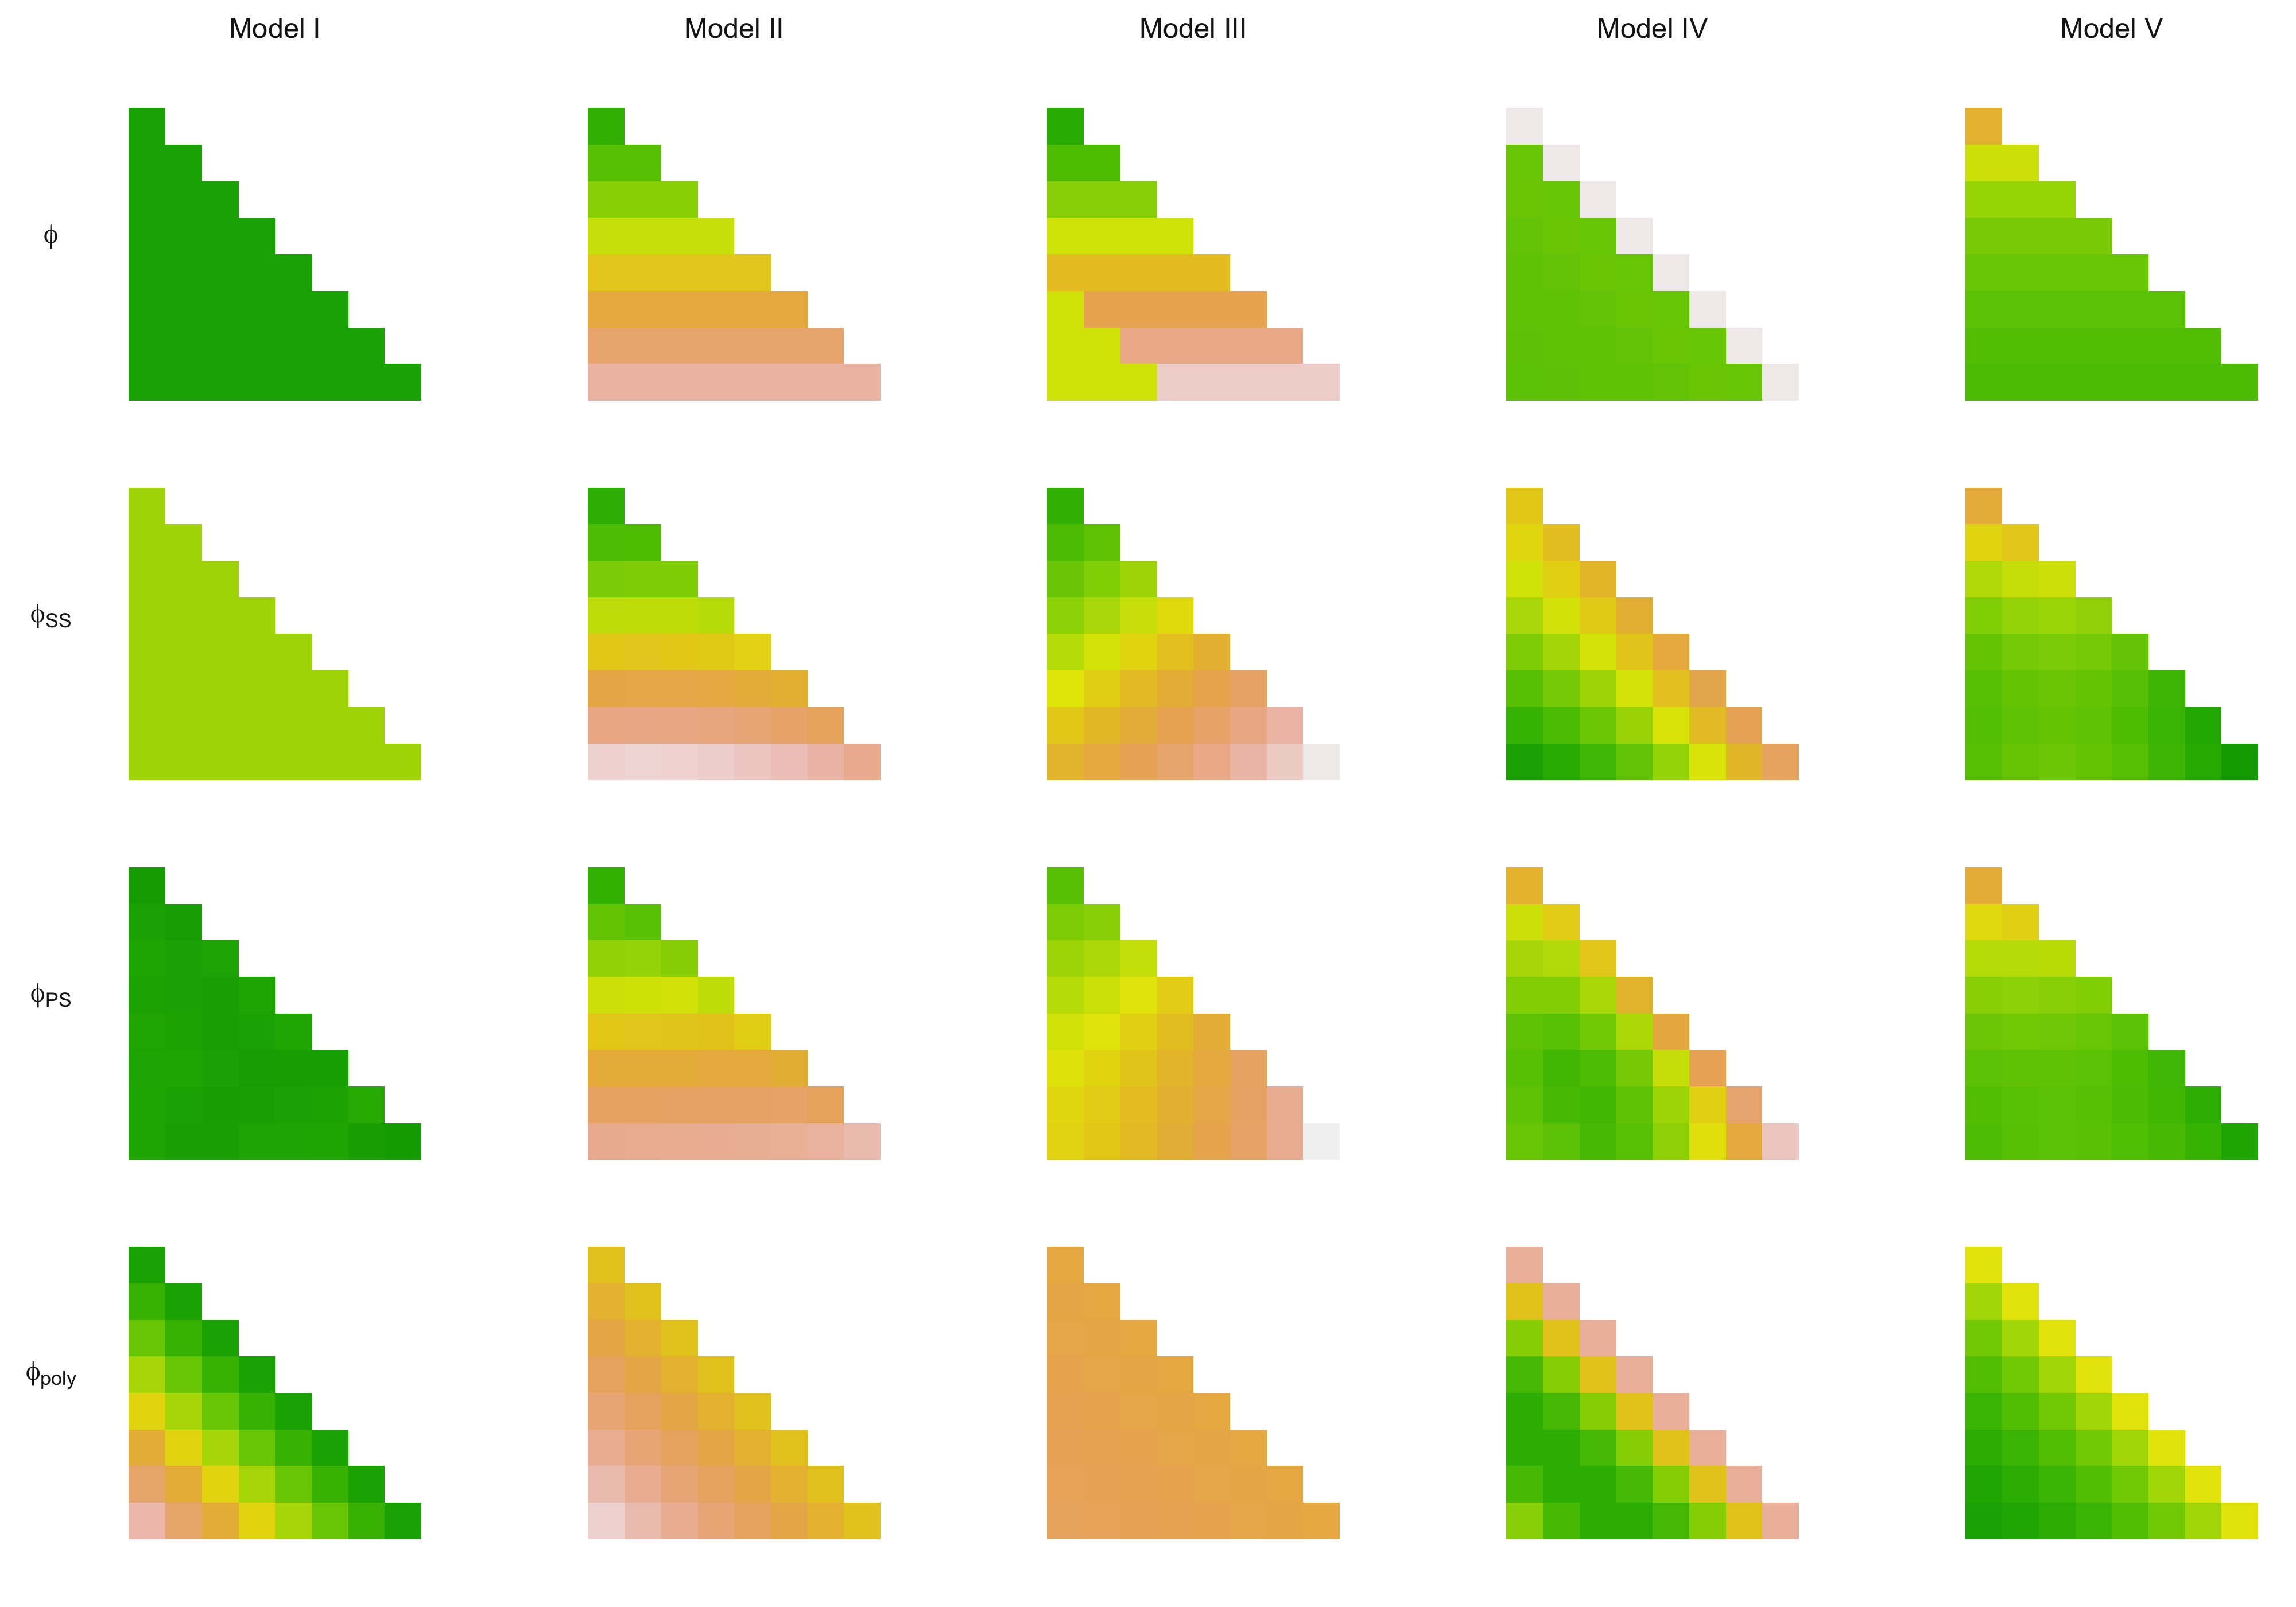
\includegraphics[width = \textwidth]{img/chapter-4/cholesky-estimate-lattice-beamer}%}
\end{center}
\end{frame}


\begin{frame}[c]{\emph{Simulation Studies}}{Results with complete data: Model I}
\centering
  \begin{tikzpicture}
    \node at (0,0) {  \includegraphics[width =0.9\textwidth]{img/chapter-4/model-1-entropy-loss-boxplots}};
\end{tikzpicture}
\end{frame}

\begin{frame}[c]{\emph{Simulation Studies}}{Results with complete data: Model I}
\centering
  \begin{tikzpicture}
    \node at (0,0) {  \includegraphics[width = 0.9\textwidth]{img/chapter-4/model-1-entropy-loss-boxplots-zoom} };
 \node at (0,3) {$\phi_{41}$};
\end{tikzpicture}
\end{frame}

\begin{frame}[c]{\emph{Simulation Studies}}{Results with complete data: Model II}
\begin{center}
  \includegraphics[width = 0.9\textwidth]{img/chapter-4/model-2-entropy-loss-boxplots-p-20}
\end{center}
\end{frame}

\begin{frame}[c]{\emph{Simulation Studies}}{Results with complete data: Model III}
\centering
  \begin{tikzpicture}
    \node at (0,0) {  \includegraphics[width = 0.9\textwidth]{img/chapter-4/model-3-entropy-loss-boxplots-zoom} };
\end{tikzpicture}
\end{frame}

\begin{frame}[c]{\emph{Simulation Studies}}{Results with complete data: Model IV}
\centering
\begin{tikzpicture}
\node at (0,0) {  \includegraphics[width = 0.9\textwidth]{img/chapter-4/model-4-entropy-loss-boxplots-zoom} };
\end{tikzpicture}
\end{frame}
\begin{frame}[c]{\emph{Simulation Studies}}{Results with complete data: Model V}
\centering
  \begin{tikzpicture}
    \node at (0,0) {  \includegraphics[width = 0.9\textwidth]{img/chapter-4/model-5-entropy-loss-boxplots-zoom} };
\end{tikzpicture}
\end{frame}

\begin{frame}[c]{\emph{Simulation Studies}}{Results with incomplete data, $N = 50$}
\centering
  \begin{tikzpicture}
    \node at (0,0) {  \includegraphics[width = 0.95\textwidth]{img/chapter-4/simulation-study-2-entropy-loss-boxplots} };

\draw[wes2] (-3.9,-.5) node {\footnotesize$p = 20$}; % Draws a circle
\draw[wes2] (-3.9,2.8) node {\footnotesize${p = 10}$}; % Draws a circle
\end{tikzpicture}

\end{frame}

\begin{frame}{\emph{Thank you!}}{For additional detail, writing, code, or questions, you can find me here:} 
\begin{tabular}{l}
tayler.a.blake@gmail.com \\
https://github.com/taylerablake/ \\
taylerablake.github.io
\end{tabular}
\end{frame}



\begin{frame}{\emph{Parametric Models for the Cholesky Decomposition}}{} \label{polynomial-mcd-model}

Pourahmadi (2000), Pan andMackenzie (2003) suggest modeling $\phi_{tj}$, $\sigma^2_{t}$ with covariates, letting 

\begin{align*}
\begin{split}  \label{eq:GARP-IV-parametric-model}
\phi_{jk} &= x'_{jk} \gamma \\
\log \sigma^2_{j} &= z'_{j}\lambda. 
\end{split}
\end{align*}

Common choices for the covariates $x_{jk}$ and $z_j$ are

\begin{align*}
x'_{jk} &= \left(1, t_j - t_k, \left(t_j - t_k\right)^2,\dots, \left(t_j - t_k\right)^{d-1}\right)', \\
z'_{j}  &= \left(1, t_j, \dots, t_j^{q-1}\right)'.
\end{align*} \label{eq:mcd-polynomial-model}
\noindent
Polynomial orders $d$ and $q$ are tuning parameters chosen by a model selection criterion (BIC, AIC).
\vspace{1cm}

\hyperlink{simulation-studies-benchmark-estimators}{\beamerskipbutton{Simulations}}

\end{frame}

\begin{frame}{\textit{Applying Elementwise Shrinkage to $S$}}{Tapering Estimators}\label{shrinkage-estimators}
	\footnotesize
	\begin{itemize}
 	\item \textbf{The Banded Sample Covariance Matrix} 
	\begin{align*}%\label{eq:variance-correlation-decomposition}
		B_k\left(S\right) = \begin{bmatrix} s_{ij} 1\left(\vert i-j \vert \le k\right) \end{bmatrix} = R_B \ast S,\quad 0 < k < p.
		\end{align*}
	\item \textbf{The Tapered Sample Covariance Matrix} 
		 	\begin{equation*}% \label{eq:cai-tapering-estimator}
			S^{\omega} =  \begin{bmatrix} \omega_{ij}^k s_{ij} \end{bmatrix},
			\end{equation*}
		where $0 < k < p$, and if $k_h = k/2$ 
		\begin{equation*}
		\omega^k_{ij} = k_h^{-1} \left[ \left( k - \vert i-j\vert\right)_+ - \left(k_h - \vert i-j\vert\right)_+ \right].
		\end{equation*}
	\item \textbf{Soft Thresholding Estimator:} 
			\begin{equation*}% \label{eq:spectral-decomposition}
			S^{\lambda} =   \begin{bmatrix} \mbox{sign}\left(s_{ij}\right) \left(s_{ij} - \lambda\right)_+ \end{bmatrix}
			\end{equation*}	\footnotesize
	\end{itemize}
\hyperlink{simulation-studies-benchmark-estimators}{\beamerskipbutton{Simulations}}
\end{frame}
